 \documentclass[11pt, a4paper,spanish]{article}
\usepackage[spanish,activeacute]{babel}
\usepackage[utf8]{inputenc}
\usepackage{caratula}
\usepackage[ruled,vlined,boxed,commentsnumbered]{algorithm2e}
\usepackage{graphicx}
\usepackage{fancyhdr}
\usepackage{amsfonts}
\usepackage{amssymb}
\usepackage{amsmath}
\usepackage{hyperref}
\usepackage{float}

%\usepackage[ruled,vlined,boxed,commentsnumbered]{algorithm2e}

% Encabezado y Pie de pagina
\pagestyle{fancy}
\fancyhf{}
%\fancyfoot[L]{\leftmark}
\fancyhead[L]{Ingeniería del Software 1}
\fancyhead[R]{Trabajo Pr\'actico 1}
\fancyfoot[R]{\thepage}


\begin{document}

% ------------ CARATULA ------------
     

        \materia{Ingeniería del Software 1}

        \submateria{1er cuatrimestre 2014}

    \titulo{Grupo 8: \\Trabajo Práctico 1}

%       \subtitulo{}

%       \fecha{9-04-2014}

    \integrante{Cangiani Agustín}{344/09}{cangiani@gmail.com}

    \integrante{Di Alessio Adrian}{631/06}{adrianalejandro86@hotmail.com}

    \integrante{Grosso Daniel}{694/08}{dgrosso@gmail.com}

    \integrante{Livorno Carla}{424/08}{carlalivorno@hotmail.com}
    
    \integrante{Pino Daniel}{556/07}{jdanielpino@gmail.com}

        \maketitle

        \pagebreak
 

% ------------ INDICE ------------

    \thispagestyle{empty}
    \tableofcontents
    \pagebreak


% ------------ DIAGRAMA CONTEXTO ------------

        


% ------------ DIAGRAMA OBJETIVOS ------------

%       \begin{subsection}{Diagrama de objectivos}
La figura \ref{fig:diagrama_objetivos} puede verse el diagrama de objetivos propuesto, que describe todos los objetivos del problema de las ciclovías.

\begin{figure}[H]
        \centering
        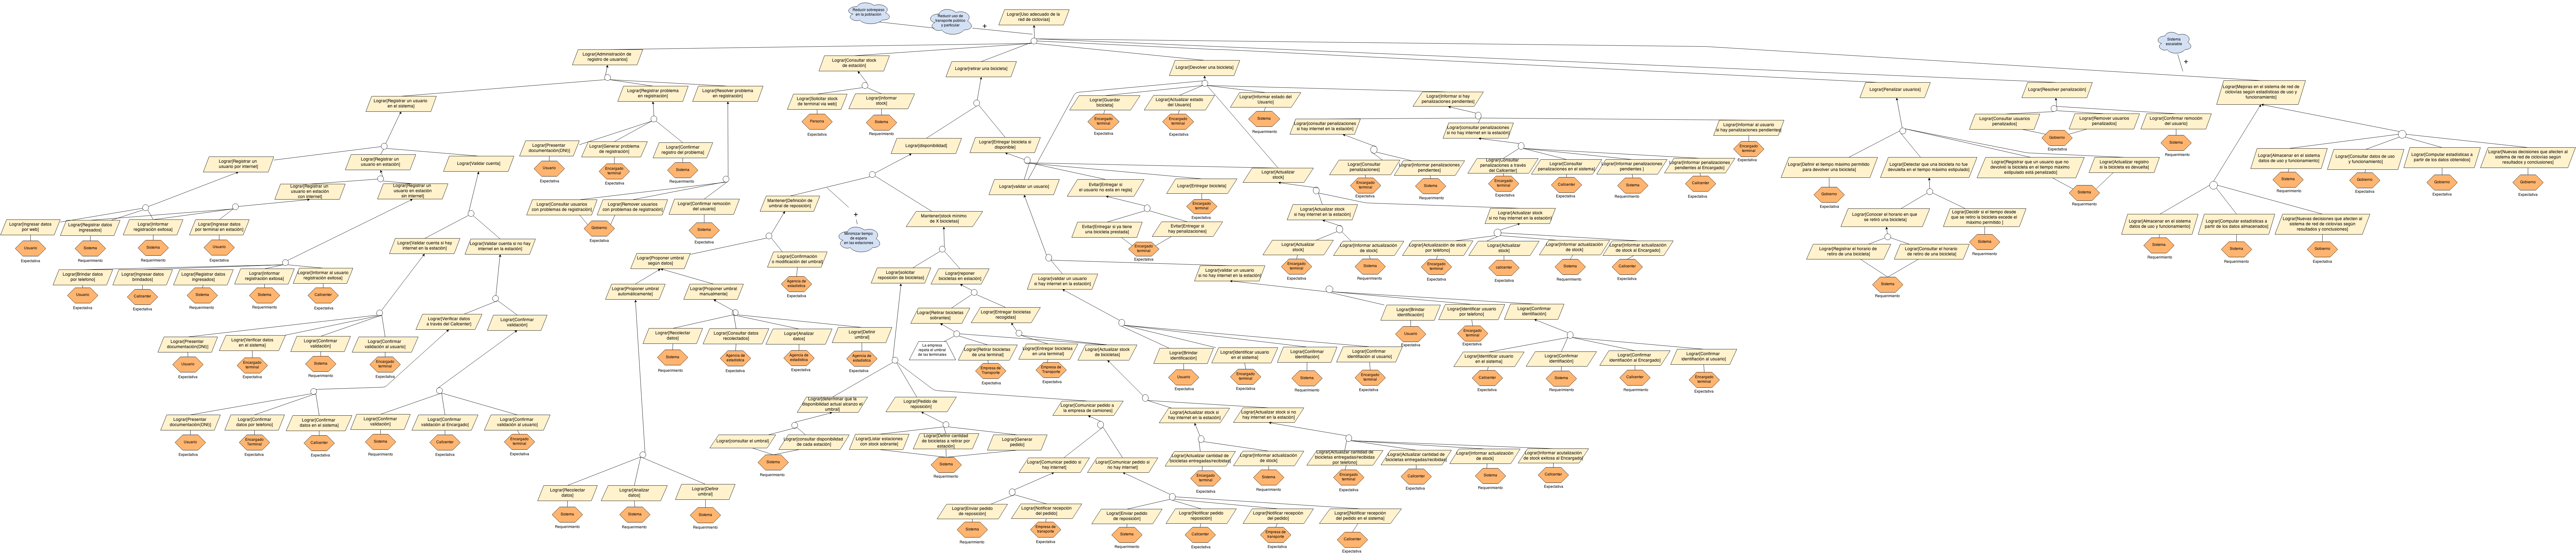
\includegraphics[angle=90,width=\textwidth,height=\textheight,keepaspectratio]{imagenes/diagrama_de_objetivos.png}
        \caption{diagrama de objetivos}
        \label{fig:diagrama_objetivos}
\end{figure}

\begin{figure}[H]
        \centering
        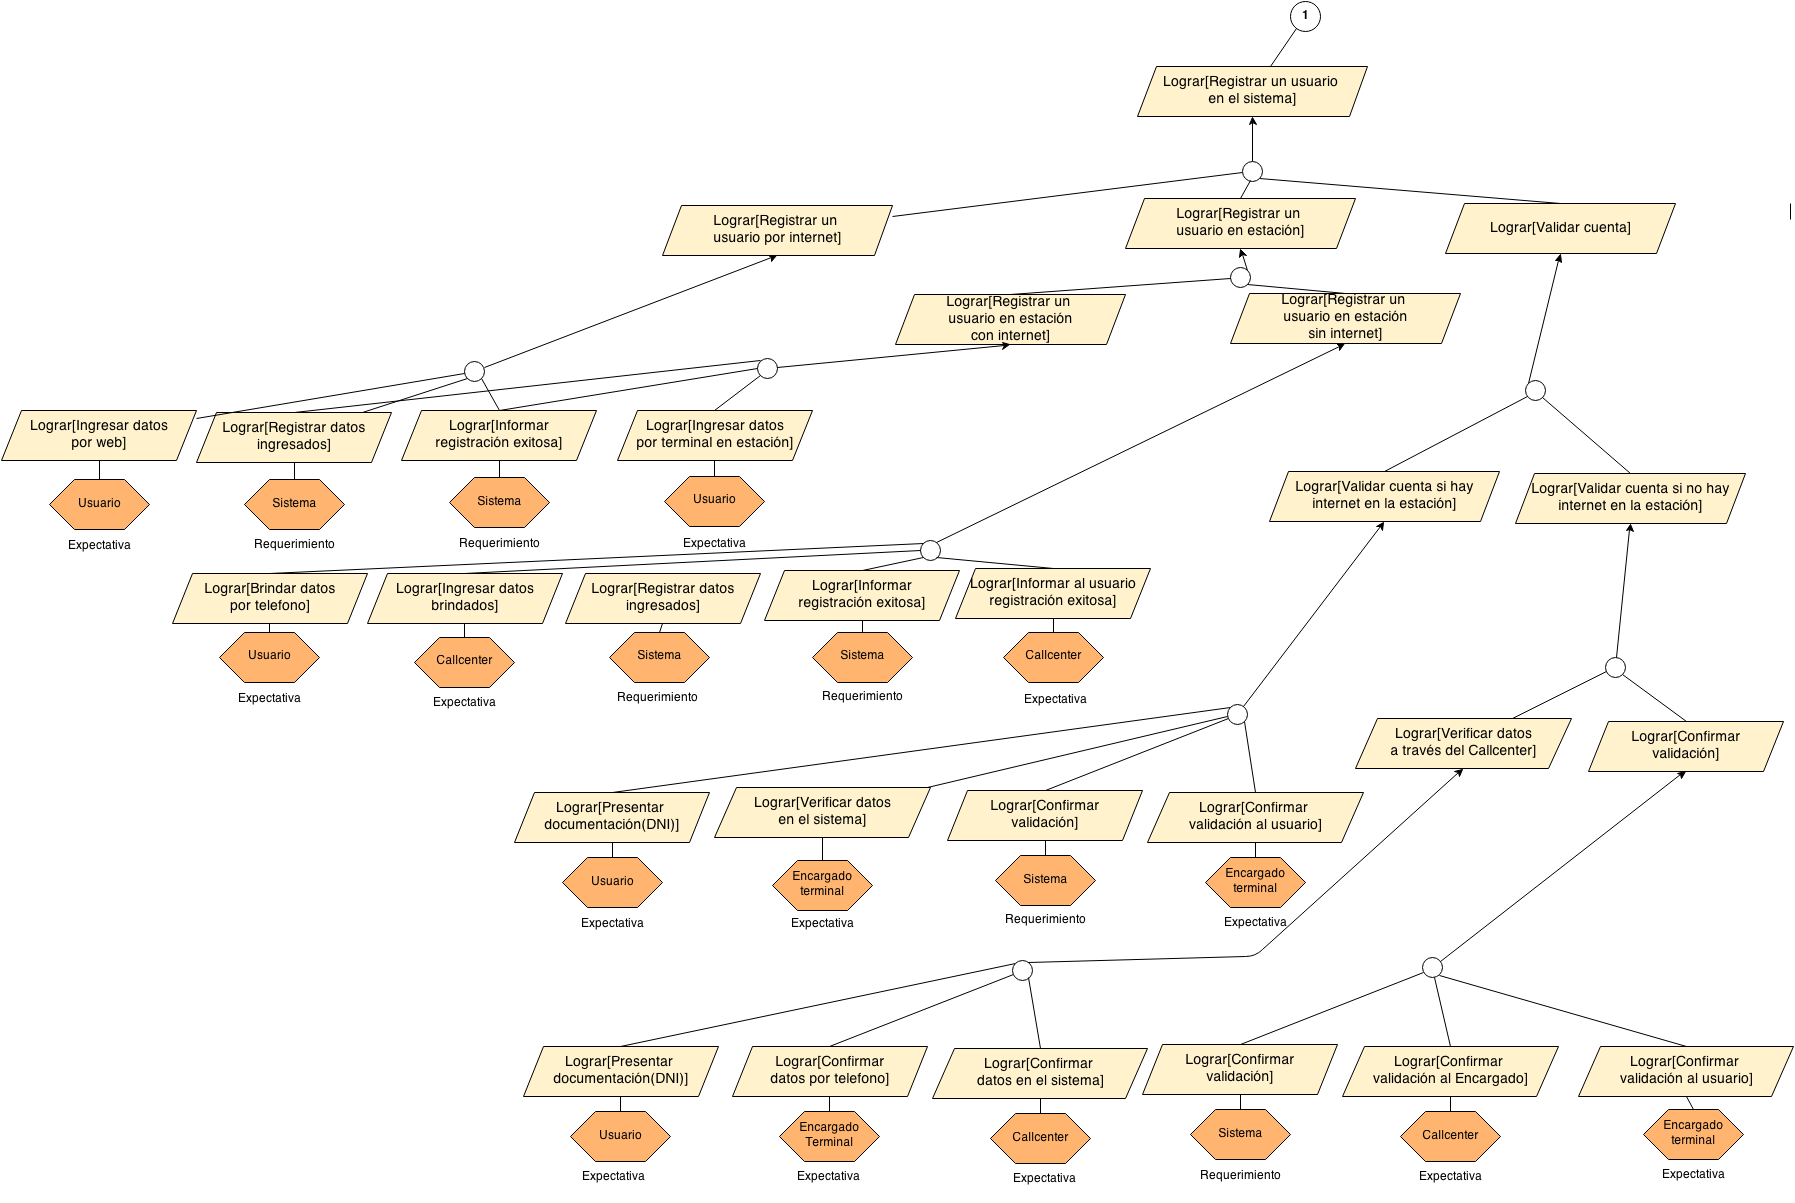
\includegraphics[angle=90,width=\textwidth,height=\textheight,keepaspectratio]{imagenes/do_1.png}
        \caption{diagrama de objetivos - 1}
        \label{fig:diagrama_objetivos_1}
\end{figure}

\begin{figure}[H]
        \centering
        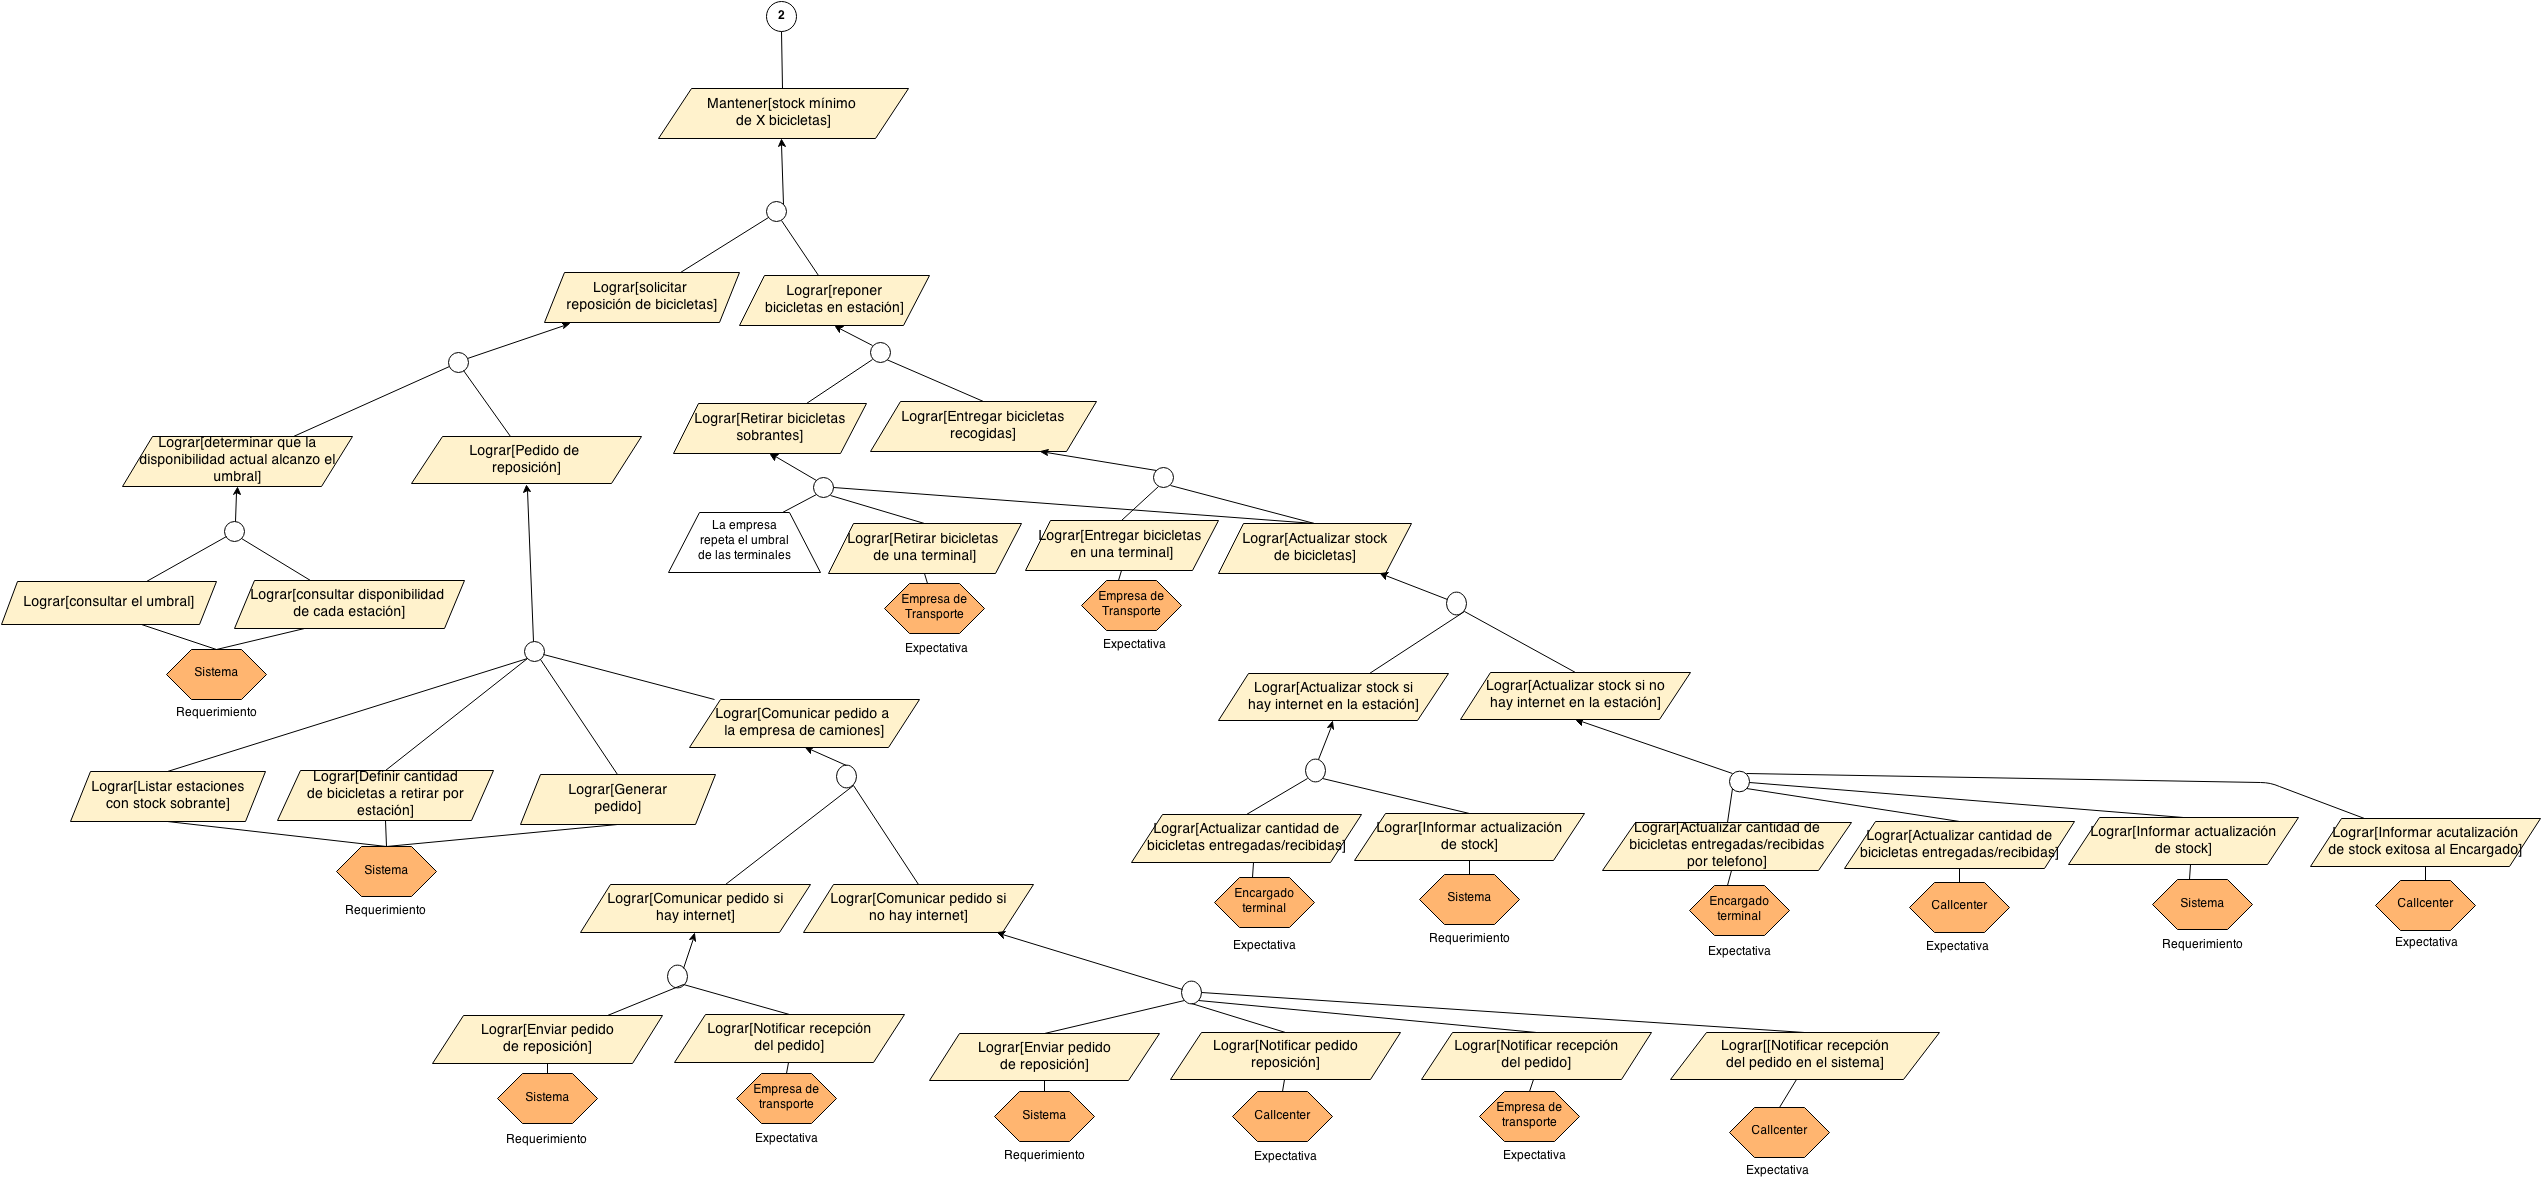
\includegraphics[angle=90,width=\textwidth,height=\textheight,keepaspectratio]{imagenes/do_2.png}
        \caption{diagrama de objetivos - 2}
        \label{fig:diagrama_objetivos_2}
\end{figure}


\begin{figure}[H]
        \centering
        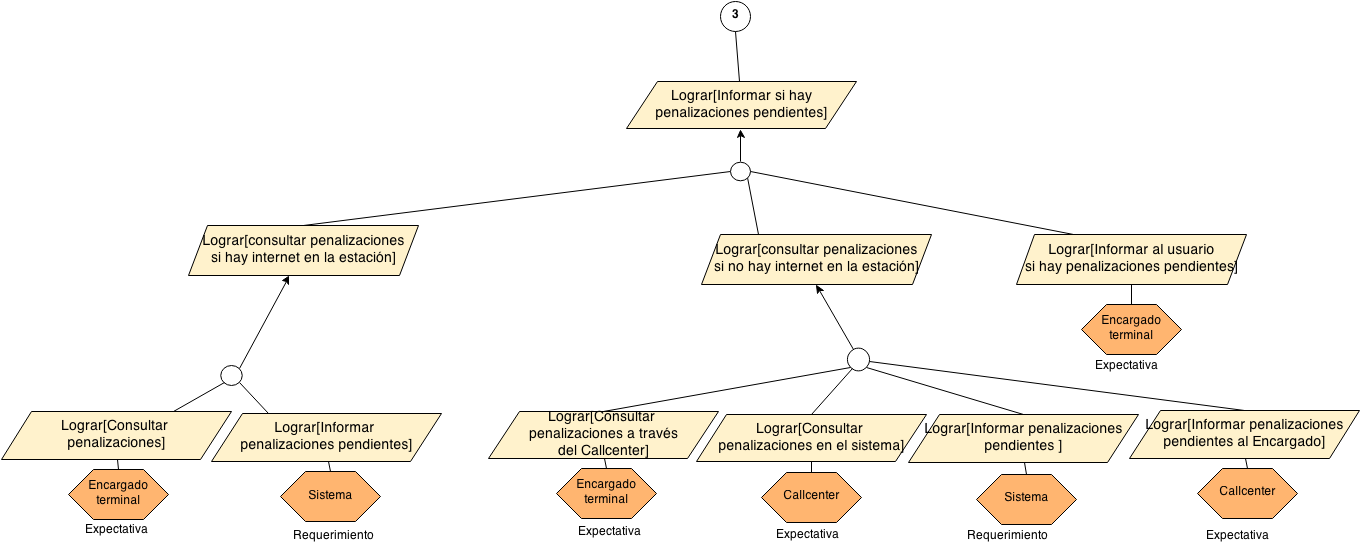
\includegraphics[angle=90,width=\textwidth,height=\textheight,keepaspectratio]{imagenes/do_3.png}
        \caption{diagrama de objetivos - 3}
        \label{fig:diagrama_objetivos_3}
\end{figure}

\begin{figure}[H]
        \centering
        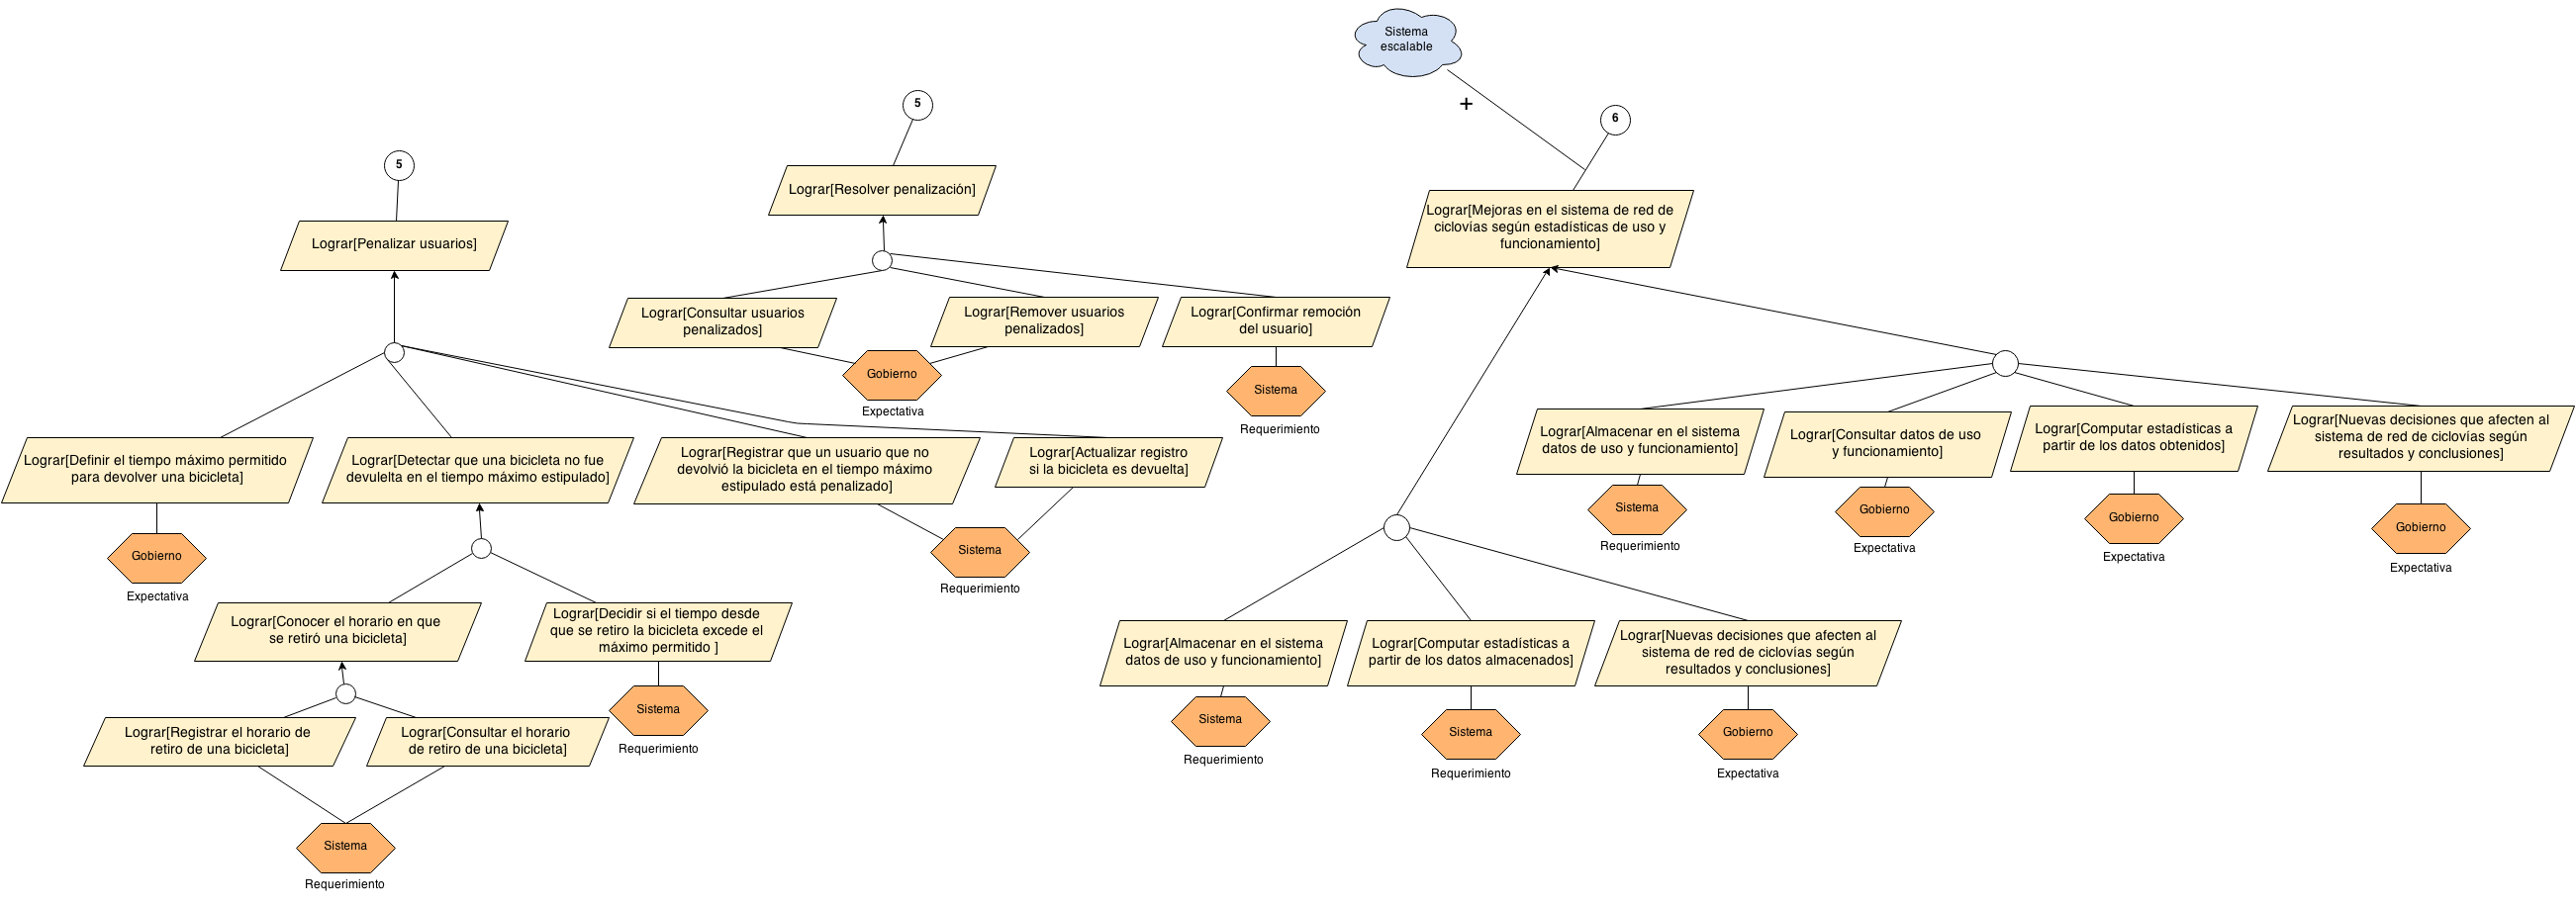
\includegraphics[angle=90,width=\textwidth,height=\textheight,keepaspectratio]{imagenes/do_4-5-6.png}
        \caption{diagrama de objetivos - 4 5 6}
        \label{fig:diagrama_objetivos_4_5_6}
\end{figure}
%\begin{figure}[H]
%	
%	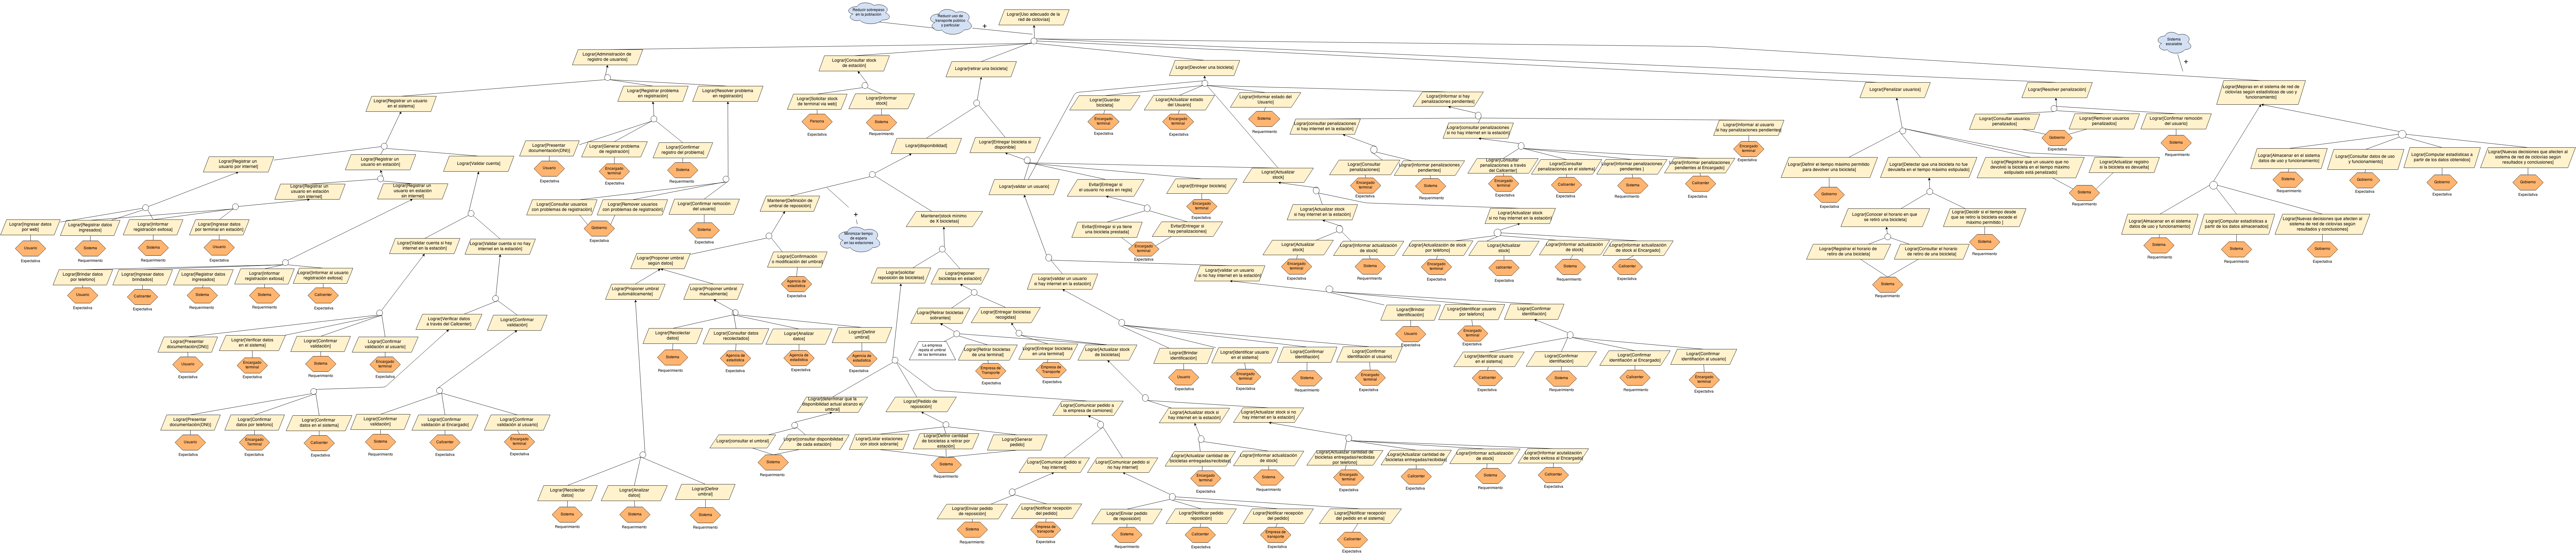
\includegraphics[scale=0.47]{imagenes/diagrama_de_objetivos.png}
%	\caption{diagrama de contexto}
%	\label{fig:diagrama_objetivos}
%
%\end{figure}

\end{subsection}

%\begin{subsection}{Análisis de objetivos}

%\end{subsection}

% ------------ REFERENCIAS ------------
    \pagebreak
%    \section{Referencias}
%        



\end{document}